\documentclass[10pt]{article}
\usepackage{icmlko}

\icmlmeta{IP 파운데이션 월드모델}{321}{셋을 통과하고도 못 벌었다}{안 쓰인 필드를 전 도메인에서 훑어 새 축을 찾았다 --- 채택 검사 셋을 다 통과했는데 유보에서 안 번다}

\begin{document}

\twocolumn[
\icmlheader

\begin{abstract}
노트 309가 \texttt{funding\_axes.category} 를 찾아 축으로 만들고 펀딩을
$+$0.117 올렸다. \textbf{같은 훑기를 전 도메인의 안 쓰인 필드에 돌렸다.}
선별기가 먼저 \textbf{아는 답 둘을 재현한다} --- \texttt{funding.category}
``새롭다''(노트 309) · \texttt{market.category} ``이미 있다''(노트 299).
새 후보가 둘 나왔다. \textbf{\texttt{webtoon.finished} 는 ①③ 을 통과하는데
사후다} --- 노트 255가 ``완결 태그가 붙은 1,271건이 전부
\texttt{finished=True}, 끝나야 붙는 표지''로 이미 배제한 것과 같은 종류다.
\textbf{선별기가 찾아도 출처가 막는다.} 남는 하나가
\texttt{anime.medium}(TVA · 극장판 · OVA)이고 \textbf{제작 단계 결정이라
사전}이다. 채택 검사 셋을 다 통과한다 --- ① $p{=}0.0084$(연도 통제 후
0.0239) · ② 시간 조각 부호 일치 \textbf{4/5} · ③ \textbf{축 스물셋을 전부
통제하고도 $H{=}35.1$}($p{<}$1e-5), 그것도 통제를 더할수록 세진다
(9.6 $\to$ 23.8 $\to$ 25.4 $\to$ 35.1). 만들어 재니 \textbf{안 번다} ---
애니 $-$0.0091($t{=}{-}1.85$)로 제 도메인이 오히려 조금 나빠지고 판은
그대로다. \textbf{왜인지는 미리 적어 뒀다} --- 학습 1,467행 중 1,382행
(\textbf{94\%})이 TVA 다. 재 보니 \textbf{최빈 무리 밖이 6\%}(유효 무리
1.32)로 판의 ``새롭다'' 38자리 중 \textbf{제일 낮다}(중앙 79\%).
\textbf{검사 넷째를 붙인다 --- 비상수성.} 다만 \textbf{필요조건이지
충분조건은 아니다}: \texttt{mkt\_cat} 은 최빈 밖 80\%인데도 $+$0.0048 이다.
\end{abstract}
]

\section{훑었더니 아는 답이 먼저 나왔다}

노트 309가 안 쓰인 필드 하나로 축을 만들었으니 \textbf{같은 훑기를 전
도메인에} 돌렸다 --- 열 개 축 파일의 모든 필드에 검사 ①③ 을 건다(모형은
안 돈다).

\begin{center}\footnotesize
\begin{tabular}{lll}
\hline
후보 & 판정 & \\
\hline
\texttt{funding.category} & 새롭다 & \textbf{노트 309가 지은 것} \\
\texttt{market.category} & 이미 있다 & \textbf{노트 299의 결론} \\
\hline
\texttt{webtoon.finished} & 새롭다 & \textbf{사후} \\
\texttt{anime.medium} & 새롭다 & 남는 하나 \\
\hline
\end{tabular}
\end{center}

\textbf{앞의 둘이 검증이다} --- 선별기가 이미 아는 답 둘을 각각 맞게 낸다.

\paragraph{\texttt{finished} 는 출처가 막는다} 웹툰 학습의 79\%가
\texttt{finished=True} 이고 라벨 중앙이 4.754 대 5.040 으로 갈린다. 그런데
노트 255가 태그 축을 만들 때 이미 적었다 --- ``완결 태그가 붙은 1,271건이
\emph{전부} \texttt{finished=True} 다. 끝나야 붙는 표지이고 노트 224가
걸러낸 것과 같은 종류다.'' \textbf{선별기는 통계만 보고 시점은 사람이
안다}(노트 306의 규약).

\section{남은 하나는 검사 셋을 다 통과한다}

\texttt{anime.medium} --- TVA(1,382) · 극장판(45) · OVA(29) · 기타(11).
\textbf{제작 단계에서 정해지고 방영 전에 안다.} 사전이다.

\begin{center}\footnotesize
\begin{tabular}{ll}
\hline
① 혼자 가르나 & $p{=}0.0084$ · 연도 통제 후 $p{=}0.0239$ \\
② 시간 조각 다섯 & 부호 일치 \textbf{4/5} \\
③ 겹침 & 축 전부(23) 통제 후 $H{=}35.1$ ($p{<}$1e-5) \\
\hline
\end{tabular}
\end{center}

\paragraph{③ 이 통제를 더할수록 세진다} 안 통제 9.6 $\to$ 공유 다섯 23.8
$\to$ 공유$+$태그 25.4 $\to$ \textbf{전부 35.1}. \textbf{기존 축이 매체를
가리고 있었다}는 뜻이다 --- 태그 축이 ``기획 시점 태그 · 장르 · 매체''에서
왔는데도 매체를 못 잡고 있었다.

무리 순서: \textbf{극장판 2.449 $>$ TVA 2.167 $>$ OVA 2.072}. 극장판이
위인 것이 이 판이 재려는 것(투자 규모와 기대)과 같은 방향이다.

\section{그런데 안 번다}

\begin{figure*}[t]
\centering
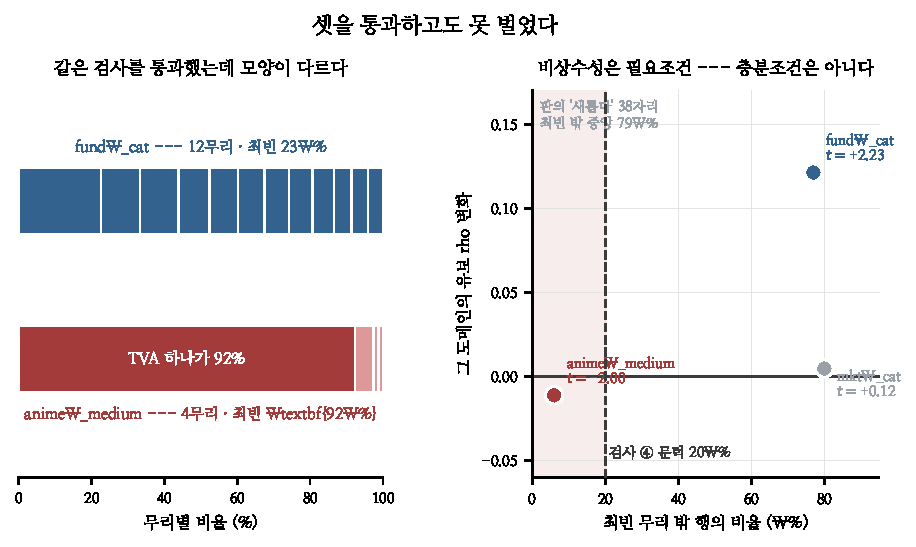
\includegraphics[width=\textwidth]{figs/const.pdf}
\caption{왼쪽 --- 두 축의 무리 분포. 오른쪽 --- 최빈 무리 밖 비율과 유보
이득.}
\end{figure*}

\begin{center}\small
\begin{tabular}{lrrl}
\hline
축 세트 & 판 차 & 애니 & \\
\hline
$+$\texttt{anime\_medium} & $+$0.0000 & \textbf{$-$0.0091} & $t{=}{-}1.85$ \\
$+$둘 다 & $-$0.0004 & $-$0.0111 & $t{=}{-}2.00$ \\
\hline
\end{tabular}
\end{center}

배포 규칙은 통과하고(판이 띠 안 · 나빠진 도메인이 문턱 안 넘음) 가드 열아홉과
표시자도 통과한다. \textbf{그런데 제 도메인이 오히려 조금 나빠진다.}

(같은 판에서 \texttt{fund\_cat} 은 펀딩 $+$0.1213($t{=}2.23$)을 유지한다 ---
새 축이 옛 축을 지우지 않았다.)

\section{미리 적어 둔 까닭이 맞았다}

\texttt{lab/animeaxes.py} 의 문서 문자열에 만들면서 적었다:
``\textbf{주의 --- 이 축은 거의 상수다. 학습 1,467행 중 1,382행(94\%)이
TVA 다. 움직일 수 있는 것은 5\%뿐이므로 이득이 작을 것이라고 미리 적는다.}''

\begin{center}\footnotesize
\begin{tabular}{lrrrl}
\hline
축 & 무리 & 최빈 밖 & 유효 무리 & 유보 \\
\hline
\texttt{fund\_cat} & 12 & \textbf{77\%} & 10.39 & $+$0.1213 \\
\texttt{mkt\_cat} & 7 & 80\% & 6.80 & $+$0.0048 \\
\texttt{anime\_medium} & 4 & \textbf{6\%} & \textbf{1.32} & $-$0.0111 \\
\hline
\end{tabular}
\end{center}

판의 ``새롭다'' \textbf{38자리}를 다 재면 최빈 무리 밖이 \textbf{중앙 79\%}
이고 \texttt{anime\_medium} 의 6\%가 \textbf{제일 낮다}(다음이 게임
\texttt{age\_rating} 14\%).

\section{검사 넷째 --- 비상수성}

\begin{center}\small
\begin{tabular}{ll}
\hline
① & 정보가 있나 \\
② & 시기에 안 흔들리나 \\
③ & 기존 축과 겹치나 \\
\textbf{④} & \textbf{충분히 많은 행을 가르나} \\
\hline
\end{tabular}
\end{center}

\texttt{lab/overlap.py} 에 넣었다 --- 최빈 무리 밖 비율과 유효 무리 수를
같이 내고 20\% 미만이면 ``거의 상수''를 세운다. \textbf{모형을 안 돌리고
계산된다} --- 지었으면 안 될 것을 짓기 전에 안다.

\paragraph{필요조건이지 충분조건이 아니다} \texttt{mkt\_cat} 은 최빈 밖
80\%인데도 $+$0.0048 이다. ④ 는 \emph{못 벌 것}을 미리 거를 뿐 \emph{벌
것}을 고르지 못한다.

\paragraph{남은 것}
\begin{center}\small
\begin{tabular}{ll}
\hline
갈래 & 왜 \\
\hline
\texttt{anime\_medium} 을 뺄까 & 애니 $-$0.009 · 문턱 아래 \\
mkt\_cat 은 왜 안 버나 & ④ 를 통과하는데 못 번다 \\
훑기를 records 로 & 축 파일 말고 원천 자료 \\
\texttt{age\_rating} & 최빈 밖 14\% --- 같은 병일 수 \\
\hline
\end{tabular}
\end{center}

\paragraph{규약} \textbf{검사를 통과한 것을 지어 보면 검사가 는다.}
채택 검사 셋은 노트 239 · 285가 정했고 오늘까지 그것으로 골랐다.
\texttt{anime\_medium} 이 셋을 다 통과하고 못 벌면서 \textbf{넷째가 생겼다}
--- 그리고 그것은 모형을 안 돌리고 계산된다. \textbf{못 번 축이 검사 하나를
낳았으면 그 축은 값을 한 셈이다.} 그리고 \textbf{미리 적어 두면 실패가
확인이 된다} --- 만들면서 ``거의 상수라 이득이 작을 것''을 적었고 그대로
됐으므로, 이것은 사후 해명이 아니라 예측이었다.

\end{document}
